\chapter{Исследовательская часть}

\section{Технические характеристики}

Технические характеристики устройства, на котором выполнялось тестирование:

\begin{itemize}
	\item Операционная система: Manjaro \cite{manjaro} Linux x86\_64.
	\item Память: 8 GiB.
	\item Процессор: Intel® Core™ i5-8265U\cite{intel}.
\end{itemize}

Тестирование проводилось на ноутбуке, включенном в сеть электропитания. Во
время тестирования ноутбук был нагружен только встроенными приложениями
окружения, окружением, а также непосредственно системой тестирования.

\section{Примеры работы программы}

В данном подразделе представлены примеры работы программы. На рисунке
\ref{img:rus} приведен пример работы программы при вводе строк в русской
раскладке и равными расстояниями Левенштейна и Дамерау-Левенштейна. На рисунке
\ref{img:eng} приведен пример работы программы при вводе строк в английской
раскладке и разными полученными значениями расстояний.

% \begin{figure}[ht!]
% \begin{center}
%     \begin{minipage}[h]{0.4\linewidth}
%         \begin{center}
%             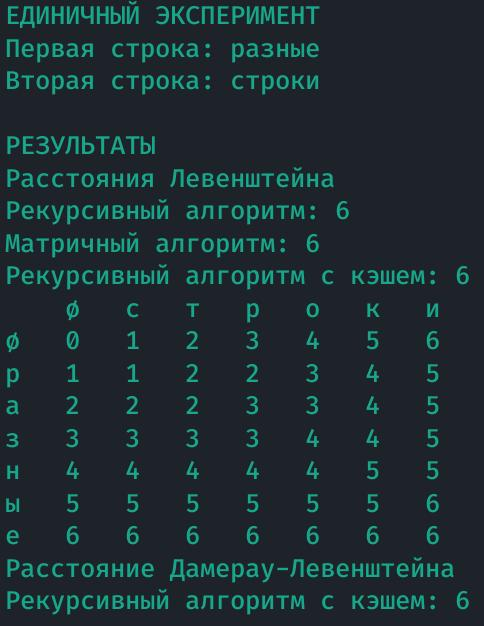
\includegraphics[height=6.5cm]{../data/img/exRus.jpg}
%             \caption{Пример работы программы в русской раскладке}
%             \label{img:rus}
%         \end{center}
%     \end{minipage}
%     \hspace{2ex}
%     \begin{minipage}[h]{0.4\linewidth}
%         \begin{center}
%             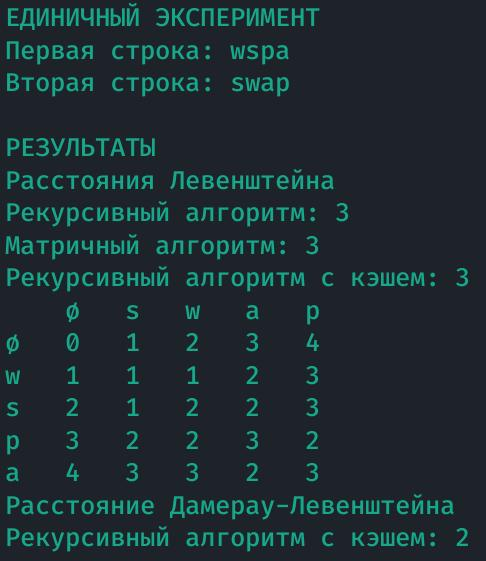
\includegraphics[height=6.5cm]{../data/img/exEng.jpg}
%             \caption{Пример работы программы в английской раскладке}
%             \label{img:eng}
%         \end{center}
%     \end{minipage}
% \end{center}
% \end{figure}

\section{Результаты тестирования}

В таблице \ref{tab:testRes} приведены результаты работы программы на тестах,
описанных в таблице \ref{tab:tests}. В результате сравнения ожидаемого и
полученного результата делаем вывод, что все тесты были пройдены.

% \begin{table}[h]
% 	\begin{center}
% 		\caption{\label{tab:testRes}Результаты тестирования}
% 		\begin{tabular}{|c|c|c|c|}
% 			\hline
% 			& & \multicolumn{2}{c|}{\bfseries Полученный результат}\\ \cline{3-4}
% 			\bfseries Строка 1  & \bfseries Строка 2 &
%             \bfseries Левенштейн & \bfseries Дамерау-Левенштейн
% 			\csvreader{../data/csv/tests.csv}{}
% 			{\\\hline \csvcoli&\csvcolii&\csvcoliii&\csvcoliv}
% 			\\\hline
% 		\end{tabular}
% 	\end{center}
% \end{table}

\section[Постановка эксперимента по замеру времени]
        {Постановка ~~эксперимента ~~по ~~замеру времени}


\section{Результаты эксперимента}

% \begin{table}[h]
% 	\begin{center}
% 		\caption{\label{tab:cmpLev}Время работы различных реализаций
%                 алгоритма поиска расстояния Левенштейна (время в наносекундах)}
% 		\begin{tabular}{|c|c|c|c|}
% 			\hline
% 			\bfseries Длина  & \bfseries Рекурсивный &
%             \bfseries Матричный & \bfseries Рекурсивный с кэшем 
% 			\csvreader{../data/csv/cmpLev.csv}{}
% 			{\\\hline \csvcoli&\csvcolii&\csvcoliii&\csvcoliv}
% 			\\\hline
% 		\end{tabular}
% 	\end{center}
% \end{table}
% \noindent
% \img{5cm}{cmpLevNT}{Графики зависимости времени выполнения алгоримтов
%                     поиска расстояния Левенштейна от длины строк}{cmpLev}
% 
% \begin{table}[h]
% 	\begin{center}
% 		\caption{\label{tab:LvsDL}Время работы алгоритмов с кэшем поиск
%                  расстояния Левенштейна и Дамерау-Левенштейна}
% 		\begin{tabular}{|c|c|c|c|}
% 			\hline
% 			\bfseries Длина  & \bfseries Левенштейн &
%             \bfseries Дамерау-Левенштейн
% 			\csvreader{../data/csv/LvsDL.csv}{}
% 			{\\\hline \csvcoli&\csvcolii&\csvcoliii}
% 			\\\hline
% 		\end{tabular}
% 	\end{center}
% \end{table}
% \clearpage
% \noindent
% \img{5cm}{LvsDLNT}{Графики зависимости времени выполнения алгоритмов с кэшем
%                    поиска расстояния Левенштейна и Дамерау-Левенштейна
%                    от длины строк}{LvsDL}

\section{Вывод}

